\documentclass{standalone}
\usepackage{tikz}
\usetikzlibrary{patterns, positioning}


\begin{document}
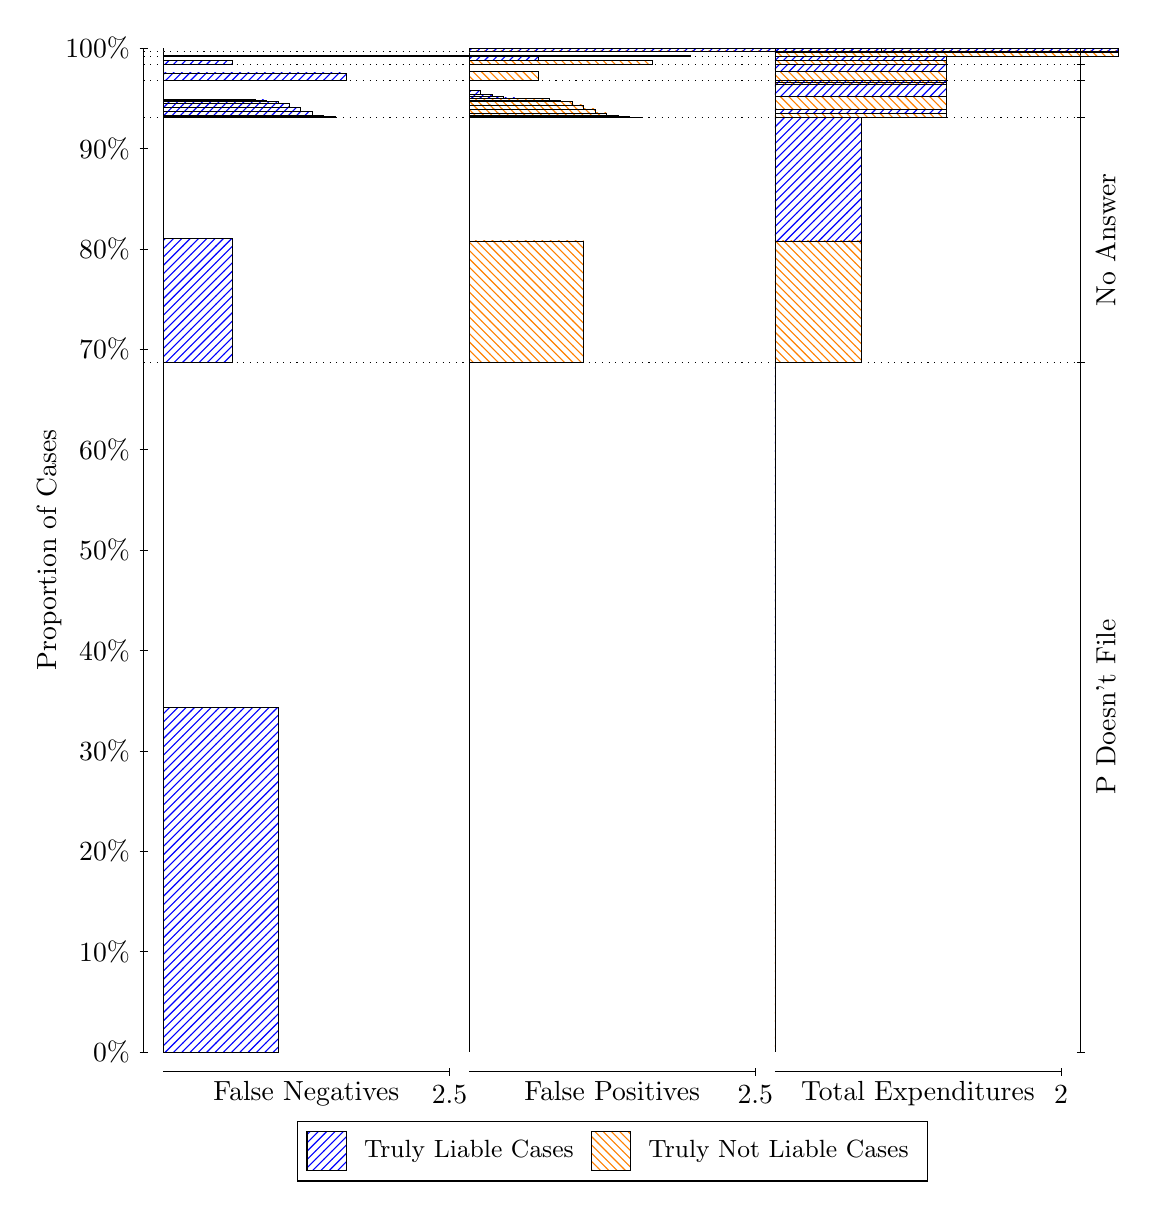
\begin{tikzpicture}
\draw[black, very thin] (1.5,1.75) -- (1.5,14.5);
\node[rotate=90, text=black, anchor=center] at (0.3, 8.125) {Proportion of Cases};
\draw[black, very thin] (1.45,1.75) -- (1.55,1.75);
\node[text=black, anchor=east] at (1.45, 1.75) {0\%};
\draw[black, very thin] (1.45,3.025) -- (1.55,3.025);
\node[text=black, anchor=east] at (1.45, 3.025) {10\%};
\draw[black, very thin] (1.45,4.3) -- (1.55,4.3);
\node[text=black, anchor=east] at (1.45, 4.3) {20\%};
\draw[black, very thin] (1.45,5.575) -- (1.55,5.575);
\node[text=black, anchor=east] at (1.45, 5.575) {30\%};
\draw[black, very thin] (1.45,6.85) -- (1.55,6.85);
\node[text=black, anchor=east] at (1.45, 6.85) {40\%};
\draw[black, very thin] (1.45,8.125) -- (1.55,8.125);
\node[text=black, anchor=east] at (1.45, 8.125) {50\%};
\draw[black, very thin] (1.45,9.4) -- (1.55,9.4);
\node[text=black, anchor=east] at (1.45, 9.4) {60\%};
\draw[black, very thin] (1.45,10.675) -- (1.55,10.675);
\node[text=black, anchor=east] at (1.45, 10.675) {70\%};
\draw[black, very thin] (1.45,11.95) -- (1.55,11.95);
\node[text=black, anchor=east] at (1.45, 11.95) {80\%};
\draw[black, very thin] (1.45,13.225) -- (1.55,13.225);
\node[text=black, anchor=east] at (1.45, 13.225) {90\%};
\draw[black, very thin] (1.45,14.5) -- (1.55,14.5);
\node[text=black, anchor=east] at (1.45, 14.5) {100\%};

\draw[black, very thin] (13.4,1.75) -- (13.4,14.5);
\draw[black, very thin] (13.35,1.75) -- (13.45,1.75);
\node[anchor=west] at (13.35, 1.75) {};
\draw[black, very thin] (13.35,10.511) -- (13.45,10.511);
\node[anchor=west] at (13.35, 10.511) {};
\draw[black, very thin] (13.35,13.618) -- (13.45,13.618);
\node[anchor=west] at (13.35, 13.618) {};
\draw[black, very thin] (13.35,14.09) -- (13.45,14.09);
\node[anchor=west] at (13.35, 14.09) {};
\draw[black, very thin] (13.35,14.293) -- (13.45,14.293);
\node[anchor=west] at (13.35, 14.293) {};
\draw[black, very thin] (13.35,14.397) -- (13.45,14.397);
\node[anchor=west] at (13.35, 14.397) {};
\draw[black, very thin] (13.35,14.453) -- (13.45,14.453);
\node[anchor=west] at (13.35, 14.453) {};
\draw[black, very thin] (13.35,14.5) -- (13.45,14.5);
\node[anchor=west] at (13.35, 14.5) {};

\draw[black, very thin, pattern color=blue, pattern=north east lines] (1.75,1.75) rectangle (3.2033,6.1303);
\draw[black, very thin, pattern color=orange, pattern=north west lines] (1.75,6.1303) rectangle (1.75,10.511);
\draw[black, very thin, pattern color=blue, pattern=north east lines] (1.75,10.511) rectangle (2.622,12.078);
\draw[black, very thin, pattern color=orange, pattern=north west lines] (1.75,12.078) rectangle (1.75,13.618);
\draw[black, very thin, pattern color=blue, pattern=north east lines] (1.75,13.618) rectangle (3.93,13.635);
\draw[black, very thin, pattern color=blue, pattern=north east lines] (1.75,13.635) rectangle (3.7847,13.646);
\draw[black, very thin, pattern color=blue, pattern=north east lines] (1.75,13.646) rectangle (3.6393,13.693);
\draw[black, very thin, pattern color=blue, pattern=north east lines] (1.75,13.693) rectangle (3.494,13.75);
\draw[black, very thin, pattern color=blue, pattern=north east lines] (1.75,13.75) rectangle (3.3487,13.801);
\draw[black, very thin, pattern color=blue, pattern=north east lines] (1.75,13.801) rectangle (3.2033,13.825);
\draw[black, very thin, pattern color=blue, pattern=north east lines] (1.75,13.825) rectangle (3.058,13.84);
\draw[black, very thin, pattern color=blue, pattern=north east lines] (1.75,13.84) rectangle (2.9127,13.846);
\draw[black, very thin, pattern color=blue, pattern=north east lines] (1.75,13.846) rectangle (2.7673,13.852);
\draw[black, very thin, pattern color=orange, pattern=north west lines] (1.75,13.852) rectangle (1.75,14.09);
\draw[black, very thin, pattern color=blue, pattern=north east lines] (1.75,14.09) rectangle (4.0753,14.183);
\draw[black, very thin, pattern color=orange, pattern=north west lines] (1.75,14.183) rectangle (1.75,14.293);
\draw[black, very thin, pattern color=blue, pattern=north east lines] (1.75,14.293) rectangle (2.622,14.347);
\draw[black, very thin, pattern color=orange, pattern=north west lines] (1.75,14.347) rectangle (1.75,14.397);
\draw[black, very thin, pattern color=blue, pattern=north east lines] (1.75,14.397) rectangle (8.4353,14.407);
\draw[black, very thin, pattern color=orange, pattern=north west lines] (1.75,14.407) rectangle (1.75,14.453);
\draw[black, very thin, pattern color=orange, pattern=north west lines] (1.75,14.453) rectangle (1.75,14.464);
\draw[black, very thin, pattern color=blue, pattern=north east lines] (1.75,14.464) rectangle (1.75,14.5);
\draw[black, very thin, pattern color=orange, pattern=north west lines] (5.6333,1.75) rectangle (5.6333,6.1304);
\draw[black, very thin, pattern color=blue, pattern=north east lines] (5.6333,6.1304) rectangle (5.6333,10.511);
\draw[black, very thin, pattern color=orange, pattern=north west lines] (5.6333,10.511) rectangle (7.0867,12.051);
\draw[black, very thin, pattern color=blue, pattern=north east lines] (5.6333,12.051) rectangle (5.6333,13.618);
\draw[black, very thin, pattern color=orange, pattern=north west lines] (5.6333,13.618) rectangle (7.8133,13.624);
\draw[black, very thin, pattern color=orange, pattern=north west lines] (5.6333,13.624) rectangle (7.668,13.631);
\draw[black, very thin, pattern color=orange, pattern=north west lines] (5.6333,13.631) rectangle (7.5227,13.649);
\draw[black, very thin, pattern color=orange, pattern=north west lines] (5.6333,13.649) rectangle (7.3773,13.675);
\draw[black, very thin, pattern color=orange, pattern=north west lines] (5.6333,13.675) rectangle (7.232,13.727);
\draw[black, very thin, pattern color=orange, pattern=north west lines] (5.6333,13.727) rectangle (7.0867,13.779);
\draw[black, very thin, pattern color=orange, pattern=north west lines] (5.6333,13.779) rectangle (6.9413,13.824);
\draw[black, very thin, pattern color=orange, pattern=north west lines] (5.6333,13.824) rectangle (6.796,13.834);
\draw[black, very thin, pattern color=orange, pattern=north west lines] (5.6333,13.834) rectangle (6.6507,13.856);
\draw[black, very thin, pattern color=blue, pattern=north east lines] (5.6333,13.856) rectangle (6.36,13.862);
\draw[black, very thin, pattern color=blue, pattern=north east lines] (5.6333,13.862) rectangle (6.2147,13.868);
\draw[black, very thin, pattern color=blue, pattern=north east lines] (5.6333,13.868) rectangle (6.0693,13.883);
\draw[black, very thin, pattern color=blue, pattern=north east lines] (5.6333,13.883) rectangle (5.924,13.907);
\draw[black, very thin, pattern color=blue, pattern=north east lines] (5.6333,13.907) rectangle (5.7787,13.958);
\draw[black, very thin, pattern color=blue, pattern=north east lines] (5.6333,13.958) rectangle (5.6333,14.09);
\draw[black, very thin, pattern color=orange, pattern=north west lines] (5.6333,14.09) rectangle (6.5053,14.201);
\draw[black, very thin, pattern color=blue, pattern=north east lines] (5.6333,14.201) rectangle (5.6333,14.293);
\draw[black, very thin, pattern color=orange, pattern=north west lines] (5.6333,14.293) rectangle (7.9587,14.343);
\draw[black, very thin, pattern color=blue, pattern=north east lines] (5.6333,14.343) rectangle (6.5053,14.397);
\draw[black, very thin, pattern color=orange, pattern=north west lines] (5.6333,14.397) rectangle (5.6333,14.443);
\draw[black, very thin, pattern color=blue, pattern=north east lines] (5.6333,14.443) rectangle (5.6333,14.453);
\draw[black, very thin, pattern color=orange, pattern=north west lines] (5.6333,14.453) rectangle (12.319,14.464);
\draw[black, very thin, pattern color=blue, pattern=north east lines] (5.6333,14.464) rectangle (10.865,14.5);
\draw[black, very thin, pattern color=orange, pattern=north west lines] (9.5167,1.75) rectangle (9.5167,6.1304);
\draw[black, very thin, pattern color=blue, pattern=north east lines] (9.5167,6.1304) rectangle (9.5167,10.511);
\draw[black, very thin, pattern color=orange, pattern=north west lines] (9.5167,10.511) rectangle (10.607,12.051);
\draw[black, very thin, pattern color=blue, pattern=north east lines] (9.5167,12.051) rectangle (10.607,13.618);
\draw[black, very thin, pattern color=orange, pattern=north west lines] (9.5167,13.618) rectangle (11.697,13.669);
\draw[black, very thin, pattern color=blue, pattern=north east lines] (9.5167,13.669) rectangle (11.697,13.721);
\draw[black, very thin, pattern color=orange, pattern=north west lines] (9.5167,13.721) rectangle (11.697,13.883);
\draw[black, very thin, pattern color=blue, pattern=north east lines] (9.5167,13.883) rectangle (11.697,14.045);
\draw[black, very thin, pattern color=orange, pattern=north west lines] (9.5167,14.045) rectangle (11.697,14.069);
\draw[black, very thin, pattern color=blue, pattern=north east lines] (9.5167,14.069) rectangle (11.697,14.09);
\draw[black, very thin, pattern color=orange, pattern=north west lines] (9.5167,14.09) rectangle (11.697,14.201);
\draw[black, very thin, pattern color=blue, pattern=north east lines] (9.5167,14.201) rectangle (11.697,14.293);
\draw[black, very thin, pattern color=orange, pattern=north west lines] (9.5167,14.293) rectangle (11.697,14.343);
\draw[black, very thin, pattern color=blue, pattern=north east lines] (9.5167,14.343) rectangle (11.697,14.397);
\draw[black, very thin, pattern color=orange, pattern=north west lines] (9.5167,14.397) rectangle (13.877,14.443);
\draw[black, very thin, pattern color=blue, pattern=north east lines] (9.5167,14.443) rectangle (13.877,14.453);
\draw[black, very thin, pattern color=orange, pattern=north west lines] (9.5167,14.453) rectangle (13.877,14.464);
\draw[black, very thin, pattern color=blue, pattern=north east lines] (9.5167,14.464) rectangle (13.877,14.5);
\draw[black, dotted] (1.5,10.511) -- (13.4,10.511);
\draw[black, dotted] (1.5,13.618) -- (13.4,13.618);
\draw[black, dotted] (1.5,14.09) -- (13.4,14.09);
\draw[black, dotted] (1.5,14.293) -- (13.4,14.293);
\draw[black, dotted] (1.5,14.397) -- (13.4,14.397);
\draw[black, dotted] (1.5,14.453) -- (13.4,14.453);
\draw[black, very thin] (1.75,1.5) -- (5.3833,1.5);
\node[text=black, anchor=north] at (3.5667, 1.5) {False Negatives};
\draw[black, very thin] (5.3833,1.45) -- (5.3833,1.55);
\node[text=black, anchor=north] at (5.3833, 1.45) {2.5};

\draw[black, very thin] (5.6333,1.5) -- (9.2667,1.5);
\node[text=black, anchor=north] at (7.45, 1.5) {False Positives};
\draw[black, very thin] (9.2667,1.45) -- (9.2667,1.55);
\node[text=black, anchor=north] at (9.2667, 1.45) {2.5};

\draw[black, very thin] (9.5167,1.5) -- (13.15,1.5);
\node[text=black, anchor=north] at (11.333, 1.5) {Total Expenditures};
\draw[black, very thin] (13.15,1.45) -- (13.15,1.55);
\node[text=black, anchor=north] at (13.15, 1.45) {2};

\node[text=black, centered, rotate=90] at (13.72, 6.1304) {P Doesn't File};
\node[text=black, centered, rotate=90] at (13.72, 12.064) {No Answer};






\draw (7.449999999999999,1.5) node[draw=none] (baseCoordinate) {};
\begin{scope}[align=center]
        \matrix[scale=0.5, draw=black, below=0.5cm of baseCoordinate, nodes={draw}, column sep=0.1cm]{
            \node[rectangle, draw, minimum width=0.5cm, minimum height=0.5cm, pattern color=blue, pattern=north east lines] {}; &
            \node[draw=none, font=\small, text=black] (B) {Truly Liable Cases}; &
            \node[rectangle, draw, minimum width=0.5cm, minimum height=0.5cm, pattern color=orange, pattern=north west lines] {}; &
            \node[draw=none, font=\small, text=black] (B) {Truly Not Liable Cases}; \\
            };
\end{scope}

\end{tikzpicture}
\end{document}